\documentclass{article}
%%
% Пакет позволяющий определить, что используется: latex или pdflatex?
%%
\usepackage{ifpdf}


%%
% Определяем, используется ли XeTex?
%%
\ifx\XeTeXversion\undefined
  %%
  % Набор пакетов для работы с графическими файлами
  %%
  \ifpdf
    \usepackage[pdftex]{graphicx}
    \usepackage{cmap}
  \else
    \usepackage{graphicx}
  \fi

\else
  %%
  % Набор пакетов для поддержки русского языка в XeLaTeX
  %%
  \usepackage[cm-default]{fontspec}
  \usepackage{xunicode}
  \usepackage{xecyr}

  % Setting default fonts
  \setmainfont{Verdana} 
\fi

%%
% Дополнительные настройки
%%
\usepackage[utf8x]{inputenc} 
\usepackage[english,russian]{babel} 
\usepackage{indentfirst}


%%
% Начало документа
%%
\begin{document}

%% Картинка
\begin{figure}
  \begin{center}
    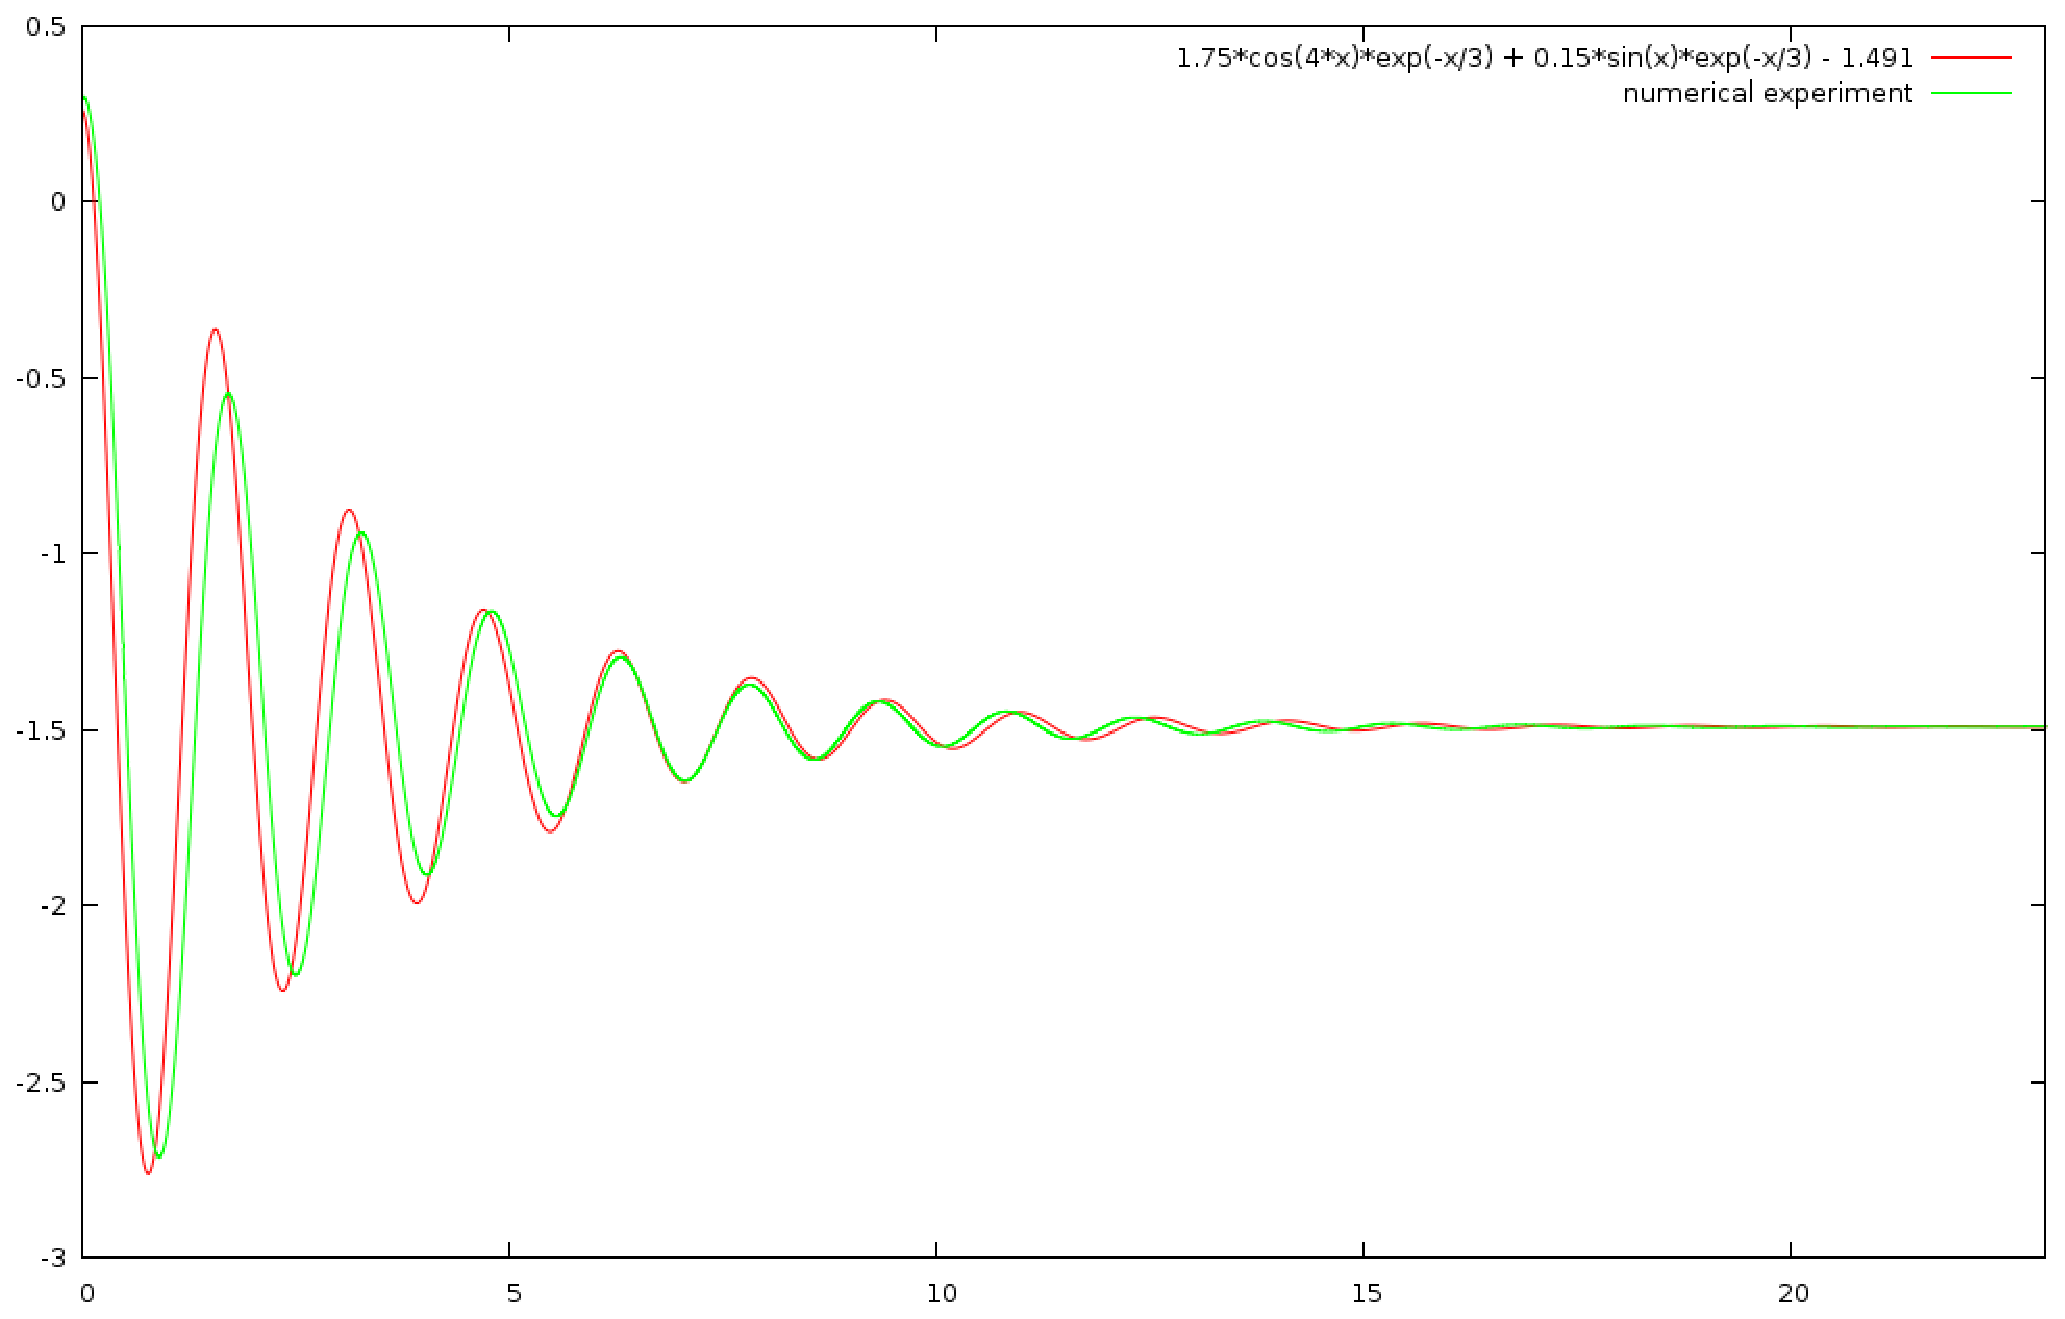
\includegraphics[width=4in,keepaspectratio]{figure1}
  \end{center}
  \caption{Моё первое изображение}
\end{figure}

%
% \begin{figure}    -- вставить плавающий объект Картинка
%   \caption{}      -- подпись к картинке
% \end{figure}
%
%
% \begin{center}    -- выравнять объект на середину страницы
% \end{center}
%
%
% \includegraphics  -- вставить графический объект
% width=4in         -- отмасштабировать объект по ширине до 4-х дюймов
% keepaspectratio   -- сохранить соотношение сторон такое же, как в исходном изображении
% figure1           -- имя графического файла (без расширения)
%

\end{document}